
%
% Settings file
%
\include{settings}	% Document settings file

%
% We use the book class
%

\documentclass[12pt]{book}

%
% The geometry package allows consistent control of page layout
%

\usepackage[paper = a4paper,         %To be shrunk to 80% when printed
			twoside,                 %Two-side mode, switches margins on
			bindingoffset = 2mm,     %Offset for binding side of page
			hmargin = 25mm,          %Left and right margin
			vmargin = 25mm,          %Top and bottom margin
			dvipdfm]
			{geometry}
%
% Font settings
%
\usepackage[T1]{fontenc}	% Activate Type 1 fonts
\usepackage{mathptmx}       % Use Times font, also for math
\usepackage[scaled]{helvet} % for sans serif fonts (\textsf{...} or \sffamiliy)
\usepackage{sectsty}        % Change section and chapter header
%\allsectionsfont{\usefont{T1}{phv}{bc}{n}\selectfont} % Set chapter/section header to narrow helvectica (arial-like)
%\usepackage[scaled]{luximono} % for monospaced fonts (\texttt{...} or \ttfamily)


%
% Packages we need
%

\usepackage{graphicx}       % Handles figures
\usepackage[utf8]{inputenc} % We want æøå
\usepackage{amsmath}
\usepackage{amsfonts}
\usepackage[mathcal]{euscript} % For calligraphy fonts
\usepackage{booktabs}       % Publication quality tables
\usepackage{setspace}       % Easy setting of line spacing
\usepackage{forloop}		% For-loops!
\usepackage[round]{natbib}  % author and names
%\usepackage[numbers,sort&compress]{natbib}  % Sort numerical keys for multiple cites
\usepackage{hypernat}       % Avoid breaking 'backref' option of hyperref package
\usepackage{float}
\usepackage[dvipsnames]{color}   % named colors
\usepackage[procnames]{listings} % beautiful listings
\usepackage{units}				 % semantically represent numbers with units
\usepackage{natbib}
\usepackage[table]{xcolor}
\usepackage[final]{pdfpages}
\usepackage{epigraph}			%for quotation
\setlength\epigraphwidth{8cm}
%\setlength\epigraphrule{0pt} %remove line in quote
\usepackage{textcomp}
\usepackage{sidecap} %for figure caption on the side
\usepackage{enumitem} % for possibility to adjust item left margin indentation

\usepackage{titlesec} %fix header fonts
\titleformat{\title}[display]
  {\normalfont\rmfamily\huge\bfseries\color{black}}
  {\chaptertitlename\ \thechapter}{20pt}{\Huge}
\titleformat{\chapter}[display]
  {\normalfont\rmfamily\huge\bfseries\color{black}}
  {\chaptertitlename\ \thechapter}{20pt}{\Huge}
\titleformat{\section}
  {\normalfont\rmfamily\Large\bfseries\color{black}}
  {\thesection}{1em}{}
\titleformat{\subsection}
  {\normalfont\rmfamily\large\bfseries\color{black}}
  {\thesubsection}{1em}{}
%\titleformat{\subsubsection}
%  {\normalfont\rmfamily\normalsize\bfseries\color{black}}
\titleformat{\paragraph}
	{\normalfont\rmfamily\normalsize\bfseries\color{black}}

% The hyperref package allows advanced hyperlinking functionality
%
\usepackage[%dvipdfmx,        % Use dvipdf driver %KD removed
			backref,         % List citing occurences in the References
			colorlinks,      % Colored links
			citecolor=black,  % Color of cite links
			linkcolor=black,  % Color of links
			urlcolor=blue,   % Color of urls
			]{hyperref}
%\newcommand{\aref}[1]{\autoref*{#1}} % Prevent links
\newcommand{\aref}[1]{\autoref{#1}} % Enable links


%
% Set fancy page header using fancyhdr package
%
\usepackage{fancyhdr}
\pagestyle{fancy}
%\pagestyle{plain}

% Ensure that the chapter and section headings are in lowercase
\setlength{\headheight}{15pt}
\renewcommand{\chaptermark}[1]{\markboth{#1}{}}
\renewcommand{\sectionmark}[1]{\markright{\thesection\ #1}}

% Delete current section for header/footer
\fancyhf{}

% Define header/footer layout
\fancyhead[LE,RO]{\bfseries\thepage}
\fancyhead[LO]{\bfseries\rightmark}
\fancyhead[RE]{\bfseries\leftmark}
\renewcommand{\headrulewidth}{0.5pt}

% make space for the rule
\fancypagestyle{plain}{
	\fancyhead{} %get rid of the headers on plain pages
	\renewcommand{\headrulewidth}{0pt} % and the line
}
\usepackage[font={small,it,rm}]{caption}
\usepackage{atveryend}
%\usepackage{thumbs}


%
% Set header height to 30pt to make room for two rows in the header
% (useful if you have very long chapter names)
%
%\headheight 30pt


%
% Include user-defined macros
%
\include{macros}

%
% TeX is very proud of its hyphenation engine, to the point where it
% hyphenates _everything_ just to show off.  Increasing penalty for
% hyphenation, and increase tolerance for underfull boxes can make
% the text easier to read, at the expense of making the text less aligned
% to the right margin
%
\hyphenpenalty=10
\tolerance=1000


% Redefine include command -> input command
%\renewcommand{\include}{\input}

% Include only these chapters
%\includeonly{introduction}


%
% Set up the frontpage, with author, title, etc
%
%{\fontsize{28}{30}\usefont{OT1}{phv}{bc}{n}\selectfont
%{\fontsize{28}{30}\usefont{T1}{phv}{bc}{n}\selectfont Exchange of water masses

%====================================================
%------------------ BEGIN DOCUMENT ------------------
%====================================================
\begin{document}

\newcommand{\blankpage}{\newpage{}\thispagestyle{empty}\mbox{}\newpage{}}
\newcommand{\HRule}{\rule{\linewidth}{0.5mm}}

\begin{titlepage}
\begin{center}
\includegraphics[width=8cm]{uib-emblem-svart} \\[0.5cm]
\paragraph*{}


\textsc{\Large Department of Physics and Technology}\\[0.5cm]
\Large Master Thesis in Nuclear Physics \\[0.4cm]
\HRule \\[0.4cm]
{ \huge \bfseries Neutron Imaging \\ with ALPIDE chips}\\[0.5cm]  %\\ sånn ca på midten}\\[0.5cm]
\HRule \\[1.0cm]



\emph{By: Lena Setterdahl}\\
\emph{Supervisor: Dieter Roherich}\\

\paragraph*{}
\end{center}
\vfill
\begin{center}
{\large \today}
\end{center}
\end{titlepage}

%Cause all references in bibtex file to appear in the 'References' section, even
%if they are not explicitly cite'ed in the document
%\nocite{*}

%Set the fontsize and baselineskip, if something other than 10 or 12 is required
\ifDownscaledFinalDoc
	\fontsize{\TextSize}{\BaseLineSkip}
	\selectfont
\fi

%Double line spacing for draft
\ifDraft
	%\doublespacing
	\singlespacing
\fi

\renewcommand{\familydefault}{\sfdefault} %KD

%--------------------------------------------------------------------------------------------------
% FRONT MATTER
%--------------------------------------------------------------------------------------------------
\frontmatter
\normalfont\rmfamily
%\include{chap/Gd}

\tableofcontents
%\listoffigures
%\lstlistoflistings

%--------------------------------------------------------------------------------------------------
% MAIN MATTER
%--------------------------------------------------------------------------------------------------
\mainmatter

%
% Main chapters
%

\chapter{Neutron Detection}
\label{chap:NeutronDetection}

%Particle Interaction with matter
%Neutron environmets
\section{Interactions of Radiaition in Matter}
\label{sect:Interaction}

%CHARGED PARTICLES
\subsection{Charged Particle Interactions}
Particles with electrical charge are subject to electromagnetic forces. Matter is made up of atoms, which composite atomic electrons and nuclei. Atomic constituents are each surrounded by an electric field and in the path of a traversing particle, causes deacceleration and divergence from its original trajectory. Energy loss mechanisms of a charged particle are:
\begin{itemize}[noitemsep]
  \item Elastic collision with atomic nuclei
	\item Elastic scattering with atomic electrons
	\item Inelastic scattering with atomic electrons
	\item Cherenkov
	\item Transition radiation
	\item Bremsstrahlung
\end{itemize}

Again, one must distinguish based on particle properties, this time, namely mass.
The mass of a "heavy" particle is one atomic unit or greater. This includes protons, alpha and other ions. That leaves electrons and positrons as "light" particles, with an atomic mass is ... Less than protons. Heavy particles (e.g. ions) are less effected by a nuclei electric field than light particles (e.g. electrons). Elastic scattering of the nuclei effect both heavy and light, however, the impact is greater for the latter.

\subsubsection{Heavy charged particles and Bethe-Bloch}
Though there are several types of interactions, heavy charged particles mainly lose energy due to inelastic collisions with outer-shell electrons. The Bethe-Bloch formula describes their average energy loss per unit length:

\begin{equation} \label{Bethe-Bloch}
  - \frac{dE}{dx} = K \rho \frac{Z}{A} \frac{z^2}{\beta^2} \left[  \ln{\frac{2 m_e c^2 \beta^2 \gamma^2 T_{max}}{I^2}} - 2\beta^2 - \delta-2\frac{C}{Z}\right]
\end{equation}

where:

\begin{equation}
  K = 2\pi N_a {r_{e}}^{2} m_e c^2 = 0.1535 MeVcm^2/g
\end{equation}

\begin{table}[H]
\rmfamily
\centering
\begin{tabular}{llll}
$r_{e}$: & classical electron & $\rho$: & density of absorbing material \\
 & radius = $2.817\times10^-13cm^2/g$ & z: & charge of incident particle in \\
$m_{e}$: & electron mass &  & unit of e \\
$N_{a}$: & Avogadro's & $\beta$ = & $p/c$ of the incident particle \\
 & number = $6.022 \times 10^{23}mol^{-1}$ & $\gamma$ = & $1/\sqrt{1-\beta^2}$ \\
$I$: & mean excitation potential & $\delta$: & density correction \\
$Z$: & atomic number of absorbing & $C$: & shell correction \\
 & material & $W_{max}$: & maximum energy transfer in a \\
$A$: & atomic weight of absorbing material &  & single collision \\

\end{tabular}
\end{table}

Noteworthy symbols in the formula are $\beta$ (representative of incident particle speed) and z (charge of incident particle).
According to bethe-bloch, $\beta = v/c$, and thus mean energy loss $dE/dx$, is inversely proportional to $v^2$, the particle speed squared. As particles slow down their speed decreases and energy deposition increases, until fully at rest. The other dependency z shows how particles of heavier charge ionize material more effectively. (rewrite)
% - - - - - - - - - - - - - - - - - - - - - - - - - - - - - - - - -
\subsubsection{Electrons}
Light particles lose energy via other interactions in addition to elastic scattering. The total energy loss is a combination of radiational and collisional loss.

    \begin{equation}
      \left(\frac{dE}{dx}\right)_{tot}=\left(\frac{dE}{dx}\right)_{col}+\left(\frac{dE}{dx}\right)_{rad}
    \end{equation}

Collisional loss can be described by modifying Bethe-Bloch. Light particles are small in mass, as per definition, and are prone to scattering. Like heavy particles, workings of collision also apply for light particles. However, Bethe-Bloch’s assumptions of large incident particle mass and non-deviating trajectory are no longer valid and must be corrected for. Moreover, in case of an incident electron, collisions occur with identical particles, atomic electrons, and the formula must account for their indistinguishability. This changes a couple of terms in Bethe-Bloch, notably maximum allowed energy transfer $W_max = \frac{T_e}{2}$ for electrons of kinetic energy $T_e$. Considering electron properties, the modified formula becomes

    \begin{equation}
        - \frac{dE}{dx} = K \rho \frac{Z}{A} \frac{1}{\beta^2}
                          \left[
                          \ln{\frac{\tau^2(\tau+2)}{2(I/m_eC^2)^2}}+F(\tau) - \delta-2\frac{C}{Z}
                          \right]
    \end{equation}

The particles kinetic energy is represented by t, in units of $mc^2$ and, for electrons,
    \begin{equation}
      F(\tau) = 1- \beta^2+\frac{\frac{\tau^2}{8}-(2r+r)\ln{2} }{(\tau+1)^2}
    \end{equation}

Light particles also lose energy by radiation. Electrons passing a nucleus experience an attractive coulomb force exerted by the nucleus positive electric field. In a curved like manner, the electrons deviate from their straight-line path and accelerate. Accelerating charged particles emit electromagnetic waves known as breaking radiation, or bremsstrahlung. Bremsstrahlung comes at a cost of diminishing particle kinetic energy. In other words, scattered electrons slow down.

An electron can lose up to 100\% of its energy in only one or two photons. Because of this, same energy electrons vary greatly in energy loss and path length.

...

Other interactions...
Range ...

\subsection{Neutron Interactions}

A neutron constitute three quarks (udd). The up (u) and down (d) quarks have charge (u: +2/3$e$, d: -1/3$e$) and mass. Together they provide the neutron with mass, energy and net charge equal to zero. Because of its intrinsic properties, a neutron is subject to three of the four fundamental forces; weak, strong and gravitational. Due to the lack of charge neutrons do not interact electromagnetically.
Like all particles with mass and energy, the neutron is affected by gravity. The weak and strong nuclear force operate between quarks and are thus relevant when considering neutrons. The strong force is responsible for holding quarks together, to form nucleons, as well as binding protons and neutrons, to form atomic nuclei. The weak force is liable for fusion reactions as well as radioactive decay of atoms. It is also the driving force of free decaying neutrons, with a lifetime of 15 min. Its force carrier, the W boson, is quite heavy. Because of this the weak interaction typically occurs much slower than other interactions. This is why the free neutron has such a long lifetime in comparison to particles prone to other decay forces (e.g. electromagnetically-decaying pions have lifetime $10^{-16}$s).
Nuclear forces operate only when interacting particles are extremely close to one another, the strong force at $10^{-15}$cm and the weak force closer still at $10^{-18}$cm. These distances are considerably small compared to the infinite range of gravity. Though the gravitational range is large, its strength relative to the strong force is negligible. Strength of the strong force also outweighs the weak, by factor $10^6$. (source? Wiki…)

A neutron may interact with matter in one of five ways:
    \begin{enumerate}[noitemsep]
      \item Elastic scattering
      \item Inelastic scattering
      \item Neutron capture
      \item Nuclear spallation
      \item Nuclear fission
    \end{enumerate}

\subsubsection{Elastic Scattering}

In particle physics, scattering refers to a particle collision which deflects the particle trajectories. After scattering the particles propagate in a different direction than before. For the process to be classified as elastic scattering the systems total kinetic energy and momentum (in the laboratory frame of reference) must be conserved.
Fig ?? illustrates a neutron on a path colliding with a target nucleus at rest. The neutron has kinetic energy $E_N$  and is heading towards the nucleus of atomic number A. During collision, kinetic energy is transferred from the neutron to the target. Elastic collisions conserve kinetic energy, energy lost by the projectile is gained by the target. After collision the recoil nucleus has energy $E_R$ and propagates θ to initial path. Recoil target gains kinetic energy $\Delta E = E_N-E_R$ and is scattered $\phi$. Angles of final trajectories must conserve momentum.
Using classical momentum and kinetic energy equations, combined with a little math, maximum nucleus recoil energy can be expressed as
      \begin{equation}
      \label{eqn:maxRecoil}
      E_R=E_N \left (\frac{A-1}{A+1}  \right )^2
      \end{equation}
and maximum energy transfer as
      \begin{equation}
      \label{eqn:maxTransfere}
      \frac{\Delta E}{E_N} =1- \left (\frac{A-1}{A+1}  \right )^2
      \end{equation}
From equation \ref{eqn:maxTransfere} it is apparent that maximum recoil energy is highest for nuclear targets of low atomic weight.


\subsubsection{Inelastic Scattering}
Similar to elastic scattering, inelastic scattering results in deflection of neutron trajectory and a recoil nucleus. In inelastic scattering, the target nucleus absorbs and reemits the neutron. In the process some kinetic energy is converted into nuclear excitation. Neutron absorption raises the nucleus to an excited energy state. The nucleus emits one or more gamma rays until it becomes stable. Angular momentum is conserved, however, kinetic energy is not.


\subsubsection{Neutron Capture}
In neutron capture an incident neutron is absorbed by the target nucleus. Nuclear atomic number increases upon absoption by one unit and consequencly undergoes nuclear compound formation. The resultant compound nucleus is either stable or unstable. The latter leads to emission of nuclear radiation, heavy ion and/or other fundamental particles. (source? Wiki?)
There are two categories of neutron capture, radiative and nonradiative. Radiative capture reactions produce an excited compound nucleus prone to de-excitation via gamma decay; one or more gamma rays are emitted until the nucleus reaches ground state.
On the other hand, nonradiative capture reactions produce a daughter nucleus accompanied by more than one neutron (since single neutrons emission reactions are considered as inelastic scattering) or charged particles like protons and alphas.
Some of the significant capture reactions for neutron detection are B-10(n,a)Li*, Li-7(n,a)H-3 and He-3(n,p)H.
Reaction equations and nomenclature of capture reactions are listed in Table ??.

The importance of capture reactions are discussed in subsection ?? and an in-depth discussion of gadolinium neutron capture is provided in subsection ??.

\subsubsection{Nuclear Spallation}
...
\subsubsection{Nuclear Fission}
Neutron induced fission is a nuclear reaction (or nuclear decay process) in which an atom absorbs a neutron and splits into two or more fission fragments. In contrast to nonradiative capture where reaction products are a heavy ion accompanied by smaller particles, fission products are comparable in size, though slightly different. Some reactions also produce neutrons which can contribute to self-sustainable fission chains.
Fission reactions release a tremendous amount of energy compared to other neutron reactions. Because of this they provide an effective method for detector neutrons, especially in high gamma environments, which becomes apparent in later chapters.


%\label{chap:NeutronDetectors}
%%----------------------------------------------------------------------
%%----------------------------------------------------------------------

Neutrons are more difficult to detected than other types of radiation. A general particle detector has a sensitive volume and when charged particles travers it they deposit some or all of their energy by ionization. Neutrons are neutral particles and do not interact electromagnetically, thus are not capable of direct ionization. A neutron reacts by hadronic forces, also known as the residual strong force. The hadronic force is a much stronger force than the electromagnetic but has a much shorter interaction range (10$^{-15}$m).  This force occurs between hadrons, for instance between a neutron and nucleons of an atom. So, while a neutron may not directly deposit its energy through ionization it can induce a nuclear reaction.  Secondary charged particles may occur from such a reaction and in turn transfer energy to the detectors sensitive volume. Neutrons can therefore be detected by combining a neutron conversion material with a general particle/radiation detector.
In principle any particle detector can be turned into a neutron detector.
A breif introduction to the most common particle detectors is in place. %?? change

...gadolinium...

\section{Basic Particle Detectors}
One of the major components of a particle detector is the sensitive volume. Incoming radiation interacts with the sensitive volume and one way or another create electrical charges responsible for a detector signal. In gas detectors this volume is, intuitively enough, filled with gas. In semiconductors a solid material fills the volume. Scintillators may incorporate material of either gas, liquid or solids, depending on detector application and requirements. Reacting with the sensitive volume, radiation may produce charge carries directly, like in gas detectors (ion pairs) and semiconductors (electron-hole pairs), or cause a process which subsequently produce charge carriers, like in scintillators (photoelectrons).

%%\paragraph{The Gas Detector} \newline
\subsection{The Gas Detector}
The basic components of a gas detector are the gas-filled chamber (i.e. sensitive volume) and electrodes (cathode and anode, i.e. the charge collectors). In general, the outer chamber-wall (cathode) is most often spherical or cylindrical and encompasses the, usually rod-shaped, anode.  A voltage is applied to the collector plates and gives rise to an electric field between the two.
When an energetic particle enters the gas-filled chamber the gas molecules are ionized. With enough energy the incoming particles can tear an electron from its atom and produce an ion pair. The electric field between the collector plates attract the newly created charges, the positive ion to the cathode (-) and electron to the anode (+).
A charged particle in an electric field experiences a force and the magnitude of its acceleration depends on the particles mass. The electrons significantly smaller mass (??) causes it to accelerate at a considerably larger rate than the heavy ion and is thus the first of the two to be collected. The speed at which charge carriers travels depends on the chamber pressure and the applied field strength.

%\paragraph{The Scintillation Detector} \newline
\subsection{The Scintillation Detector}
...
%\paragraph{The Semiconductor Detector} \newline
\subsection{The Semiconductor Detector}
...


These detectors are initially oblivious to non-ionizing radiation such as neutrons. However, by incorporating a converter material to the design it allows for indirect detection thereof.

\section{Reactions of Neutron Detection}

\subsection{Neutron Energies Dependence}
Neutrons reaction probability with matter is heavily dependent on its energy and are categorized into four regions. Slow neutrons have energies 0-0.4 MeV and their reaction probability drop inversely with their speed. The intermediate neutron energy range is the interval 0.4-200keV. Many reactions have resonances in this interval, and it is therefore also known as the resonance region. Most neutrons, however, are created with a much larger energy and are labeled as fast neutrons, 200 keV-20 MeV. Lastly, neutrons energies beyond 20MeV are known as high energy neutrons. High neutrons exceed the scope of this thesis and will not be discussed any further.
Neutron reaction cross-section is much higher in the slow and intermediate domain than the fast and high domain. As the neutron speed v increases from slow to intermediate, many reaction probabilities decrease proportionally to 1/v. Once the energy reaches the domain of intermediate neutrons a number of reactions experience resonance. Moving into the fast neutron region, the likelihood of nuclear reactions lessens, and the probability of elastic scattering takes over.
Elastic scattering is widely used in detection of fast neutrons. The interaction produces no secondary particles, but rather results in a recoil nucleus which is responsible for ionizing the detector medium. Fast neutrons have a tendency to scatter more easily of atoms, especially those with a low atomic number such as hydrogen (Ref. on elastic scattering of hydrogen?).

\subsection{Reaction Characteristics}
To ensure good quality neutron signals the conversion material must meet certain standards. First and foremost, it is essential that the material possesses a high probability of neutron interaction. The ideal situation would be 100\% neutron detection, no neutrons going unseen. Nevertheless, this is usually not the case since some neutrons pass through the conversion material unaffected or react in other non-signal generating ways. High neutron reaction probability is therefore an essential characteristic of the conversion material to ensure a high detection efficiency.

Another important trait of a neutron detector is gamma discrimination. Often, neutrons are accompanied by gamma-radiation, to which neutron detectors have a similar response. This makes the identification of neutrons somewhat more difficult. Reactions with a high Q-value yield highly energetic particles and produce high signals. In comparison, energy deposited by gamma-rays are much lower. Incorporating conversion materials based on high Q reactions is one way to better distinguishing neutron from gamma signals. In intense gamma-fields, however, the accumulation of photon signals can become a problem.


\subsection{Popular reactions}
Popular nuclear reactions used to convert a neutron into signal inducing radiation are exoergic reactions and radiative capture. Typical nuclear reactions used in neutron detection are B-10(n,a)Li-7, Li-6(n,a)T, He-3(n,p)T and Gd(n,γ)Gd*. The first three classified as exoergic reactions and the last one as radiative capture.
An exoergic reaction is a nuclear reaction with a positive Q-value. This means the reaction products have a higher kinetic energy than the incident particle. These reactions commonly exhibit a high reaction probability for thermal neutrons and produce high energy and easily detectable particles.
Radiative capture is a reaction in which an incident neutron is absorbed by the target nucleus and forms a compound nucleus that decays to its ground state through radiative decay. The probability of absorption is large for thermal neutrons in heavy material and the probability of competing reactions, like elastic scattering, is small. \newline

%\noindent{\bf B-10(n,a)Li-7} \newline
%\noindent
Probably one of the most popular reactions in the detection of slow/thermal neutrons is the {\bf B-10(n,a)Li-7} reaction. The most probable outcome of the reaction dominates 94\% of the capture events and produces a Li-7* nucleus in its first excited state and an alpha particle. The remaining six per cent lead to the same reaction products, the only difference being Li-7 in ground state and higher reaction energy.
In nearly all events a 480 keV gamma is emit by the excited nucleus. Since neutron detectors are also gamma sensitive these gamma-rays are often of value and can be used as neutron indicators along with the emitted alpha particle (google this?).
A particularly attractive trait of B-10 is its high cross-section of 3840 barns at thermal energies, as well as the reaction products short range and high energy deposit such that gamma induced signals are relatively small. Even more interesting, B-10 comes in many different compound forms, making it an extremely versatile element of neutron measurements. As a gas, it is frequently used in BF3- filled proportional counters; as a solid, it can be applied as a lining to proportional-counters filled with a common proportional-counter gas; and as an oxide, incorporated in zinc sulfide in scintillators or dissolved as methyl borate in organic scintillators. The list goes on.
At higher neutron energies the reaction equation changes substantially. The branching ratio begins to even out and the fraction of events producing gamma shrink from 94\% to 33\%. Furthermore, at neutron energies 5-10 MeV other secondary particles can be produced, e.g. proton, deuterons and tritons, as observed by Frye and Gammel in 1956 (9). These effects, however, are not of great concern as the reaction cross sections are low and B-10 is not used in fast neutron detection. \newline

%\noindent{\bf Li-6(n,a)T} \newline
%\noindent
The {\bf Li-6(n,a)T} reactions cross section is 940 barns for thermal energies and decreases with neutron energy until it exhibits resonance in the intermediate range around 250keV.  Similar to B-10(n,a)Li-7, its thermal cross section is proportional to the inverse speed of the incident neutron.
Though the cross section is less than that of B-10, a higher reaction energy, which helps distinguish reaction particles from gamma rays, is at its advantage.
Lithium is widely available in various forms but exhibits no solid compounds applicable for neutron detection and is therefore less versatile than boron. For slow neutron detecting scintillators, Li-6(n,a)T is the most commonly used nuclear reaction. \newline

%\noindent{\bf He-3(n,p)T} \newline
%\noindent
A reaction which has long been the mainstay of neutron detection is {\bf He-3(n,p)T}.
He-3 is a noble gas and, when of sufficient purity, it is well suited as a counting gas. Its high thermal cross section of 5330 barns makes it a very attractive conversion material and is therefore preferred in applications requiring high detection efficiency. Despite having a high detection probability, the Q-value is small and makes gamma-discrimination considerably more difficult than for boron-enriched BF3 proportional counters.
Stock supplies of He-3 were in good shape up until the years following the attack of September 9th, 2001. Prices of He-3 skyrocketed along with the demands on nuclear security resulting in a worldwide shortage thereof (AMBIGIUOUS!!). Although He-3 cross section exceeds that of B-10(n,a)Li-7, its relatively high cost often hinders it from being used. The search for new alternative neutron detection methods have therefore become a popular topic within the scientific community of nuclear instrumentation (Dumarezt?). \newline

%\noindent{\bf Neutron capture in Gd} \newline
%\noindent
In recent decades, gadolinium (Gd) has been proposed as an alternative to He-3 proportional counters. Historically gadolinium is known as a neutron poison due to its high neutron absorption characteristics. Neutron capture in gadolinium is a nuclear reaction categorized as radiative capture.
In consideration of neutron detection, gadolinium is a very attractive converter material due to its huge absorption cross-section for thermal neutrons. The gadolinium isotope Gd-157 has in fact the largest cross-section for any known stable isotope of a whopping 254000 barns. That is ?? times larger than the thermal reaction probability of He-3! The most common gadolinium isotopes used in neutron conversion are Gd-155 and Gd-157 for their high reaction probability. The abundance of Gd-155 and Gd-157 is \% and \%, respectively.
Their reaction equations are:

Not only do the capture reactions possess a high probability for thermal neutrons, they also yield a significant amount of energy. This energy is released in the form of gamma-transitions and gives rise to prompt gamma-rays and electrons, i.e. signal generating radiation.


%\paragraph{TEST}

%\input{chap/NeuttronDetection/NeutronReactions}
%%\label{chap:NeutronDetectors}
%%----------------------------------------------------------------------
%%----------------------------------------------------------------------

Neutrons are more difficult to detected than other types of radiation. A general particle detector has a sensitive volume and when charged particles travers it they deposit some or all of their energy by ionization. Neutrons are neutral particles and do not interact electromagnetically, thus are not capable of direct ionization. A neutron reacts by hadronic forces, also known as the residual strong force. The hadronic force is a much stronger force than the electromagnetic but has a much shorter interaction range (10$^{-15}$m).  This force occurs between hadrons, for instance between a neutron and nucleons of an atom. So, while a neutron may not directly deposit its energy through ionization it can induce a nuclear reaction.  Secondary charged particles may occur from such a reaction and in turn transfer energy to the detectors sensitive volume. Neutrons can therefore be detected by combining a neutron conversion material with a general particle/radiation detector.
In principle any particle detector can be turned into a neutron detector.
A breif introduction to the most common particle detectors is in place. %?? change

...gadolinium...

\section{Basic Particle Detectors}
One of the major components of a particle detector is the sensitive volume. Incoming radiation interacts with the sensitive volume and one way or another create electrical charges responsible for a detector signal. In gas detectors this volume is, intuitively enough, filled with gas. In semiconductors a solid material fills the volume. Scintillators may incorporate material of either gas, liquid or solids, depending on detector application and requirements. Reacting with the sensitive volume, radiation may produce charge carries directly, like in gas detectors (ion pairs) and semiconductors (electron-hole pairs), or cause a process which subsequently produce charge carriers, like in scintillators (photoelectrons).

%%\paragraph{The Gas Detector} \newline
\subsection{The Gas Detector}
The basic components of a gas detector are the gas-filled chamber (i.e. sensitive volume) and electrodes (cathode and anode, i.e. the charge collectors). In general, the outer chamber-wall (cathode) is most often spherical or cylindrical and encompasses the, usually rod-shaped, anode.  A voltage is applied to the collector plates and gives rise to an electric field between the two.
When an energetic particle enters the gas-filled chamber the gas molecules are ionized. With enough energy the incoming particles can tear an electron from its atom and produce an ion pair. The electric field between the collector plates attract the newly created charges, the positive ion to the cathode (-) and electron to the anode (+).
A charged particle in an electric field experiences a force and the magnitude of its acceleration depends on the particles mass. The electrons significantly smaller mass (??) causes it to accelerate at a considerably larger rate than the heavy ion and is thus the first of the two to be collected. The speed at which charge carriers travels depends on the chamber pressure and the applied field strength.

%\paragraph{The Scintillation Detector} \newline
\subsection{The Scintillation Detector}
...
%\paragraph{The Semiconductor Detector} \newline
\subsection{The Semiconductor Detector}
...


These detectors are initially oblivious to non-ionizing radiation such as neutrons. However, by incorporating a converter material to the design it allows for indirect detection thereof.

\section{Reactions of Neutron Detection}

\subsection{Neutron Energies Dependence}
Neutrons reaction probability with matter is heavily dependent on its energy and are categorized into four regions. Slow neutrons have energies 0-0.4 MeV and their reaction probability drop inversely with their speed. The intermediate neutron energy range is the interval 0.4-200keV. Many reactions have resonances in this interval, and it is therefore also known as the resonance region. Most neutrons, however, are created with a much larger energy and are labeled as fast neutrons, 200 keV-20 MeV. Lastly, neutrons energies beyond 20MeV are known as high energy neutrons. High neutrons exceed the scope of this thesis and will not be discussed any further.
Neutron reaction cross-section is much higher in the slow and intermediate domain than the fast and high domain. As the neutron speed v increases from slow to intermediate, many reaction probabilities decrease proportionally to 1/v. Once the energy reaches the domain of intermediate neutrons a number of reactions experience resonance. Moving into the fast neutron region, the likelihood of nuclear reactions lessens, and the probability of elastic scattering takes over.
Elastic scattering is widely used in detection of fast neutrons. The interaction produces no secondary particles, but rather results in a recoil nucleus which is responsible for ionizing the detector medium. Fast neutrons have a tendency to scatter more easily of atoms, especially those with a low atomic number such as hydrogen (Ref. on elastic scattering of hydrogen?).

\subsection{Reaction Characteristics}
To ensure good quality neutron signals the conversion material must meet certain standards. First and foremost, it is essential that the material possesses a high probability of neutron interaction. The ideal situation would be 100\% neutron detection, no neutrons going unseen. Nevertheless, this is usually not the case since some neutrons pass through the conversion material unaffected or react in other non-signal generating ways. High neutron reaction probability is therefore an essential characteristic of the conversion material to ensure a high detection efficiency.

Another important trait of a neutron detector is gamma discrimination. Often, neutrons are accompanied by gamma-radiation, to which neutron detectors have a similar response. This makes the identification of neutrons somewhat more difficult. Reactions with a high Q-value yield highly energetic particles and produce high signals. In comparison, energy deposited by gamma-rays are much lower. Incorporating conversion materials based on high Q reactions is one way to better distinguishing neutron from gamma signals. In intense gamma-fields, however, the accumulation of photon signals can become a problem.


\subsection{Popular reactions}
Popular nuclear reactions used to convert a neutron into signal inducing radiation are exoergic reactions and radiative capture. Typical nuclear reactions used in neutron detection are B-10(n,a)Li-7, Li-6(n,a)T, He-3(n,p)T and Gd(n,γ)Gd*. The first three classified as exoergic reactions and the last one as radiative capture.
An exoergic reaction is a nuclear reaction with a positive Q-value. This means the reaction products have a higher kinetic energy than the incident particle. These reactions commonly exhibit a high reaction probability for thermal neutrons and produce high energy and easily detectable particles.
Radiative capture is a reaction in which an incident neutron is absorbed by the target nucleus and forms a compound nucleus that decays to its ground state through radiative decay. The probability of absorption is large for thermal neutrons in heavy material and the probability of competing reactions, like elastic scattering, is small. \newline

%\noindent{\bf B-10(n,a)Li-7} \newline
%\noindent
Probably one of the most popular reactions in the detection of slow/thermal neutrons is the {\bf B-10(n,a)Li-7} reaction. The most probable outcome of the reaction dominates 94\% of the capture events and produces a Li-7* nucleus in its first excited state and an alpha particle. The remaining six per cent lead to the same reaction products, the only difference being Li-7 in ground state and higher reaction energy.
In nearly all events a 480 keV gamma is emit by the excited nucleus. Since neutron detectors are also gamma sensitive these gamma-rays are often of value and can be used as neutron indicators along with the emitted alpha particle (google this?).
A particularly attractive trait of B-10 is its high cross-section of 3840 barns at thermal energies, as well as the reaction products short range and high energy deposit such that gamma induced signals are relatively small. Even more interesting, B-10 comes in many different compound forms, making it an extremely versatile element of neutron measurements. As a gas, it is frequently used in BF3- filled proportional counters; as a solid, it can be applied as a lining to proportional-counters filled with a common proportional-counter gas; and as an oxide, incorporated in zinc sulfide in scintillators or dissolved as methyl borate in organic scintillators. The list goes on.
At higher neutron energies the reaction equation changes substantially. The branching ratio begins to even out and the fraction of events producing gamma shrink from 94\% to 33\%. Furthermore, at neutron energies 5-10 MeV other secondary particles can be produced, e.g. proton, deuterons and tritons, as observed by Frye and Gammel in 1956 (9). These effects, however, are not of great concern as the reaction cross sections are low and B-10 is not used in fast neutron detection. \newline

%\noindent{\bf Li-6(n,a)T} \newline
%\noindent
The {\bf Li-6(n,a)T} reactions cross section is 940 barns for thermal energies and decreases with neutron energy until it exhibits resonance in the intermediate range around 250keV.  Similar to B-10(n,a)Li-7, its thermal cross section is proportional to the inverse speed of the incident neutron.
Though the cross section is less than that of B-10, a higher reaction energy, which helps distinguish reaction particles from gamma rays, is at its advantage.
Lithium is widely available in various forms but exhibits no solid compounds applicable for neutron detection and is therefore less versatile than boron. For slow neutron detecting scintillators, Li-6(n,a)T is the most commonly used nuclear reaction. \newline

%\noindent{\bf He-3(n,p)T} \newline
%\noindent
A reaction which has long been the mainstay of neutron detection is {\bf He-3(n,p)T}.
He-3 is a noble gas and, when of sufficient purity, it is well suited as a counting gas. Its high thermal cross section of 5330 barns makes it a very attractive conversion material and is therefore preferred in applications requiring high detection efficiency. Despite having a high detection probability, the Q-value is small and makes gamma-discrimination considerably more difficult than for boron-enriched BF3 proportional counters.
Stock supplies of He-3 were in good shape up until the years following the attack of September 9th, 2001. Prices of He-3 skyrocketed along with the demands on nuclear security resulting in a worldwide shortage thereof (AMBIGIUOUS!!). Although He-3 cross section exceeds that of B-10(n,a)Li-7, its relatively high cost often hinders it from being used. The search for new alternative neutron detection methods have therefore become a popular topic within the scientific community of nuclear instrumentation (Dumarezt?). \newline

%\noindent{\bf Neutron capture in Gd} \newline
%\noindent
In recent decades, gadolinium (Gd) has been proposed as an alternative to He-3 proportional counters. Historically gadolinium is known as a neutron poison due to its high neutron absorption characteristics. Neutron capture in gadolinium is a nuclear reaction categorized as radiative capture.
In consideration of neutron detection, gadolinium is a very attractive converter material due to its huge absorption cross-section for thermal neutrons. The gadolinium isotope Gd-157 has in fact the largest cross-section for any known stable isotope of a whopping 254000 barns. That is ?? times larger than the thermal reaction probability of He-3! The most common gadolinium isotopes used in neutron conversion are Gd-155 and Gd-157 for their high reaction probability. The abundance of Gd-155 and Gd-157 is \% and \%, respectively.
Their reaction equations are:

Not only do the capture reactions possess a high probability for thermal neutrons, they also yield a significant amount of energy. This energy is released in the form of gamma-transitions and gives rise to prompt gamma-rays and electrons, i.e. signal generating radiation.


%\paragraph{TEST}

\section{Gadolinium: as a Neutron Converter Material}
%\label{chap:GdFoil}

%%----------------------------------------------------------------------
%%----------------------------------------------------------------------
%\section{Gadolinium}

%Introduction to Gd
Gadolinium (Gd) is a chemical element with atomic number 64. It is a metal and appears as a solid under standard pressure and room temperature. In nature Gd occurs as a composition of seven isotopes; the most abundant being Gd-158 (24.84\%), followed by Gd-160 (21.86\%), Gd-156 (20.47\%), Gd-157 (15.67\%) and Gd-157 (14.80\%).

%Gd Cross section and its use
Gd has many favorable characteristics allowing an eclectic range of use; for instance in alloys to make magnets, electronics and data storage disks( *); and as a contrast agent in MRI, to diagnose cancerous tumors(*).
Of particular interest is its high neutron absorption cross section, high probability of neutron capture. Of all known natural occurring nuclei, Gd-157 has the highest neutron absorption cross section having resonance at thermal-neutron energies (*). As efficient neutron absorbers, Gd plays an important role in neutron shielding alloys for nuclear reactor safety and storage (*). An additional use of great Gd neutron capture is as Gd-based neutron poison, for instance Gd(III) nitrate in moderator systems for regulating power generation and shut-down of Heavy Water Nuclear Reactors (* page 31).
Not limited to the field of nuclear physics, Gd neutron absorption capability also benefit(s?) neutron capture therapy for cancer treatment and neutron detection, due to reaction products following neutron capture.  In gadolinium neutron capture therapy (GdNCT) a cancer patient is injected with Gd endused tracer followed by exposure to a neutron beam. Neutron absorbed by the Gd tracer produce secondary particles such as photons and electrons. While traversing tissue, the particles deposits dose and The particles travels the tissue exposed to a neutron beam, once Gd absorbs neutrons, decays and release product particles the particles  is injected to the cancer patient product particles deposits dose locally to

%Introduction to neutron detection???

%Neutron capture in gadolinium
Neutron capture cross section of natural Gd is given by the weighted sum of isotopic cross sections. Relative abundance of Gd isotopes in natural Gd and their neutron capture cross section are listed in table 1. Isotopes Gd-157 and Gd-155 collectively contribute 99.99\% of the cross section, resulting in 48800±150 barns. Natural Gd interaction with thermal neutrons may therefore be simplified as a “two-absorbing isotope system” consisting of the isotopes Gd155 and Gd157 [Dumazert, 2018].

%Nuclear reaction equation ...

Since natural Gd interaction with neutrons can be ascribed to isotopes Gd-157 and Gd-155, it is worth studying their corresponding nuclear reaction equation.

\begin{equation}
    _{64}^{155}Gd \rightarrow _{64}^{156}Gd^* \rightarrow _{64}^{156}Gd + \gamma + ICe^-     (Q=8.5 MeV)
\end{equation}
\begin{equation}
    _{64}^{157}Gd \rightarrow _{64}^{158}Gd^* \rightarrow _{64}^{158}Gd + \gamma + ICe^-    (Q=7.9 MeV)
\end{equation}

Once a Gd nuclei has absorbed a neutron it exists in an excited energy state from which it decays by gamma-transition, resulting primarily in gamma-ray ($\gamma$-ray) emission and internal conversion (IC) electrons. Byproducts of the decay are Auger and Coster-Kronig (ACK) electrons and X-rays, prompted by vacancies left by the IC electrons, for further explanation of gamma-transition see section ??. The Q-value ($Q$) is defines as the difference in mass before and after a nuclear reaction and represents the net energy released when the nuclei has decayed completely. This energy is distributed as kinetic energy among product particles. Due to the Gd nuclei’s large mass, compared to a photon (massless) and an electron, the recoil energy is neglectable ( Modern Nuclear Chemistry, page 219*). I.e. most of the Q-value is distributed among gamma-rays and IC electrons.


\subsection{Reaction Energy Spectrum}
From Gd(n,gamma) capture, the excitation energy is distributed among reaction products; roughly 99\% of the energy is carried by prompt gamma-rays and the rest by low energy electrons [Sakurai et al.]. The energy spectrum ranges from 0 MeV to the Q-value of the nuclear reaction. Energies of prompt gamma-rays lie all over the spectrum, while energies of IC electrons and their biproducts are mainly located at the lower end, below 0.2 MeV.
The resulting spectrum is an overlap of two basic components. The first is a continuous spectrum, generated by prompt gamma-rays in the medium to high energy range, and the second is a set of discrete lines, produced by low energy prompt gamma-rays, IC electrons, Auger electrons and X-rays. In other words, prompt gamma-ray emission adds to both components, while the remaining reaction products supply just the discrete.

  \begin{figure}[h]
  \centering
  	\includegraphics[width=7cm]{fig/lvl.png}
  	\caption{Nuclear levels of an arbitrary nucleus}
  	\label{fig:1}
  \end{figure}

The spectrums form is closely related to the nuclear structure of gadolinium. Figure ? illustrates excited states of an arbitrary nucleus. A low-lying level has less excitation energy than a high lying level. Low-lying levels are easily distinguishable, each with a known spin and parity, they are discrete. As the excitation energy increases so does the nuclear level density, until high lying levels eventually become indistinguishable from one another and resemble a continuum. In fig. ?, the quasicontinuum domain of energy states is represented by a gradient, where energy level density increases as the gradient darkens. Energy levels within the quasicontinuum are marked by dotted lines and the discrete domain with uninterrupted lines. There is no clear boundary between the continuous and discrete domain, but rather a smooth transition between the two. The highest energy level represents neutron capture state and the lowest level ground state, both are indicated by a bold uninterrupted line. A transition from one level to another is indicated by and arrow.

\subsubsection{Prompt Gamma-Rays}

A nucleus may transition once or several times before it reaches ground state.
Transitions can occur between (1) states in the continuous domain, (2) states in the discrete domain or (3) between the two. In the continuous domain there are nearly endless possible states from which a nucleus can decay.  It is the transitions with initial states in this domain that bring about the spectrum’s apparent continuity.
In the spectrum, gamma-rays take the form of a broad peak structure along with a couple of prominent spikes. The distribution stretches from one end of the spectrum to the other. The broad peak favors energies in the bottom half of the spectrum, its apex between 0 and 2 MeV, and tapers off slowly as it approaches maximum energy release.

As the nucleus de-excites and gets closer to ground state transitions between states in the discrete domain occurs. There is a limited amount of discrete levels, consequently the number of possible gamma-emission energies are finite, in contrast to the continuum. This results in discrete peaks near the lowest part of the energy spectrum.

\begin{figure}
  \centering
  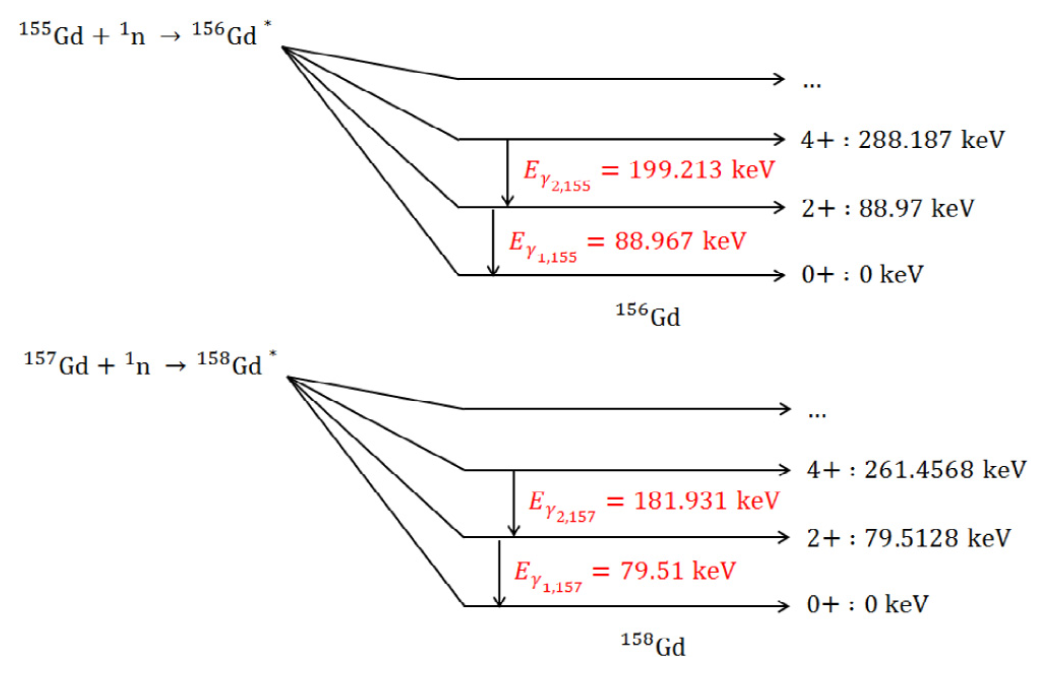
\includegraphics[width=7cm]{fig/Gd_ExcitedStates.png}
  \caption{Excitation levels of Gd-155* and Gd-157* and corrosponding gamma-transitions}
  \label{fig:1}
\end{figure}

Fig. \ref{fig:Gd_ExcitedStates} illustrates gamma-transistions associated with excited gadolinium nuclei. Two peaks, in the lower end, dominate the spectrum. In a purely isotopic material of either Gd-156* or Gd-158* a set of two energy pairs is emitted, {88.97 keV, 199.22 keV} and {79.51 keV, 181.94 keV}, respectively. The lowest energy of each set is characteristic for the transition between first excited state with spin-parity ( J^π)  2$^+$  and ground state 0$^+$, while the larger energy is characteristic for transitions between second excited state with spin-parity 4$^+$ state and first excited state 2$^+$[C.W. Reich, Nuclear Data Sheets for A = 156, Nucl. Data Sheets 113 (11) (2012) 2537–2840.]. Gamma-ray emission rate probability (per neutron capture) of Gd-157 and Gd-155 for are listed in table ?? [Gräfe et. al]

%%----------------------------------------------------------------------
\subsubsection{Internal Conversion Electrons}
%\textbf{Internal Conversion Electrons}\\
Alternatively, the atom can de-excite by means of internal conversion (IC), the direct emission of an orbital electron. In gadolinium excited by neutron capture, IC is most probable for transitions from first state to ground state $(2^+ \rightarrow 0^+)$ and second state to first state $(4^+ \rightarrow 2^+)$. These transitions are responsible for 96.7\% of the energy carried by IC electrons [??!]. They also happen to be the same transitions from which the discrete gamma-ray duplets, mentioned previously, are produced.

IC and gamma emission are competing decay modes. The ratio of IC decay rate $\lambda_{ICe^-}$ to gamma decay rate $\lambda_{\gamma}$ can be described by the internal conversion coefficient (ICC) $\alpha$:

  \begin{equation}
      \alpha =  \frac{\lambda_{ICe^-}}{\lambda_{\gamma}}
  \end{equation}

In cases where gamma decay is preferred the coefficient is small, perhaps even negligible, and differently when IC is preferred the coefficient is large.

The probability of IC depends on the electron shell (K,L, M, …)and shells therefor have respective coefficients ($\alpha_K$,$\alpha_L$,$\alpha_M$, …).

Inner shell electrons, such as those from the K shell, are more likely to interact directly with the nucleus, since its wavefunction has finite probability of penetrating the nucleus. The probability of IC in a shell becomes less likely the further away it lies from the nucleus. In other words, internal conversion depends heavily on the atomic electron density inside the nucleus. (studie of the probability of IC from shells [ref?], table?). Consequently, odds of nuclear interaction with the K-shell is more likely than with the L-shell, than the M-shell and so on.

The total ICC is the ratio of total number of IC electrons to gamma-rays emitted by a nucleus and it can be expressed as a sum of shell coefficients:

\begin{equation}
    \alpha_{TOT} =  \sum_i \alpha_i \ , \ i = K, L, M, ...
\end{equation}

Transition levels of lower energy favor internal conversion. As calculated by [A.AHarms, Table 4], transitions of Gd-157* from the second lowest transition level, L-shell of the first excited state, are 3 times more likely of mediation by IC than gamma-emission. While de-excitation from higher states are less prone to IC. Already at the third excitation state, Gd-157* exhibits a low coefficient of 0.1, meaning IC electron rates are 10 times lower than gamma rates.

The energy of an IC electron is determined by the available transition energy and the binding energy of a shell.

  \begin{equation}
      E_{ICe^- }=E_T-E_{bi,i},\ , \ i = K, L, M, ...
  \end{equation}

IC electrons contribute to discrete lines in the 20-200 keV range. Eminent is the intensity at which specifically 71 keV electrons are produced, nearly 0.27 nc$^-1$ in natural gadolinium [T.Aoyama].

%%----------------------------------------------------------------------
\subsubsection{X-rays and Auger Electrons}
When a conversion electron is expelled from subshell m a vacancy is left behind. Still in an excited state, the atom undergoes further de-excitation. An electron from a higher subshell p (>n) descends and fills the vacancy, releasing atomic excitation energy by either emission of x-rays or Auger electrons.
X-ray emission occurs when the transition energy goes into electromagnetic radiation. Difference in binding energy makes up the x-ray energy.

  \begin{equation}
      E_{x-ray} = E_T = E_{bi,p}-E_{bi,m}
  \end{equation}

On the other hand, the transition energy may go into freeing an electron of an intermediate subshell n where n lies between shell m and p. The so-called Auger electron has energy equal to the difference in transition energy and binding energy.

\begin{equation}
    E_{Ae^-} = E_T-E_{bi,n}
\end{equation}

 X-rays and Auger electrons, from L- and K-shell, of gadolinium-neutron capture are radiated in the 0-50 keV range. The most prominent x-ray has energy of 43 keV and an emission rate of 0.47 nc$^-1$ (per neutron capture). Auger electrons worth noting are of energy 35 keV (0.08 nc$^-$) and 5 keV (0.21 nc$^-1$). In comparison to x-rays, they are less frequent and of lower energies. [Dumartez]

%%----------------------------------------------------------------------
%%----------------------------------------------------------------------


\chapter{Semiconductors and Pixel Sensors}
\label{chap:SemiPixel}


%semiconductors
\section{Semiconductors}


\subsection{Energy Band Diagram}
\ref{sec:BandDiagram}
An energy band diagram is often used to illustrate the conductive properties of an atomic structure. The vertical axis corresponds total energy of an atomic electron. The horizontal axis corresponds to the position in space in the atomic structure. Valence electrons have energies indicated by the valence band (bottom band). Free electrons that are responsible for conduction lie in the conduction band (top band). Fermi energy level represents the maximum electron energy at absolute zero temperature (0K) and lies in-between the two bands. In diagrams, the area within the bands are usually shaded to indicate allowed electron energy states. The energy bands may or may not overlap. In the latter case, there is a gap between the bands which contains forbidden electron energies. This gap it is called the band-gap. The width of the band-gap ΔE is the difference between the lowest energy in the conduction band $E_C$ and the highest energy in the valence band $E_V$. A valence electron must collect energy no lesser than ΔE to enter the conduction band.

An insulator is a poor conductive material that does not conduct electric current. Its energy diagram shows that the gap between the energy bands are large. In fact, it is so large that electrons have great difficulty crossing the forbidden region and ever entering the conduction band.
In contrast, a conductor is a highly conductive material that readily allows the flow of electric current. The valence and conduction band overlap and create a union. There is no band-gap and electrons may flow freely from one band to the other.

A semiconductor is a material whose conductivity lies between an insulators and a conductors. The conductivity depends on its temperature and composite material. Rising temperatures increase the kinetic energy of valence electrons and determine whether they have enough energy to leap over the band-gap and into the conduction band. At low temperatures a semiconductor behaves like an insulator and with increasing temperatures the conductivity rises, eventually resembling that of a conductor. The conductive properties can also be altered by doping the material with impurities. Such semiconductors are called doped or extrinsic semiconductors.


\subsection{Doped Semiconductors}
When speaking about semiconductors, doping is the process of injecting impurities into the structure. Adding impurities to a pure semiconductor alters its electrical conductivity by introducing allowed energy states in the band-gap. These impurity states appear close to either the conduction band or valence band depending on the impurity. The number of valence electrons of an impurity atom determines the doping type. Semiconductors in which added impurity atoms has an extra electron are n-type while those with impurity atoms an electron short are p-type.

The most common semiconductor material is silicon (Si). Silicon belongs in group IV of the periodic table and thus has four electrons in its outer shell. In a pure silicon crystal structure, the four outer electrons each form a covalent bond with a neighboring electron of another Si-atom. At thermal equilibrium the only accepted energy states are in the valence band. If sufficient energy, at minimum the band-gap, is transferred to valence electrons they may excite to the conduction band.

A neutrally charged phosphorous (P) atom has five valence electrons, one more than Si-atoms, and as an impurity in the Si-crystal lattice acts as an electron donor. Four out of its five electrons form covalent bonds with valence electron of neighboring Si-atoms. The fifth donor electron is left loosely bound to the P-atom and, thus, is more easily excited to the conduction band.

In contrast, a neutrally charged boron (B) atom has three valence electrons. While phosphorous supplies electrons, a boron impurity contributes to electron vacancies (or holes). The holes in the Si-structure acts as electron acceptors. Valence electrons may fill a hole and, in its wake, leave a new hole. One could also say the two charge carriers (interchange?) switch positions

Figure ?? illustrates the energy band diagram of doped semiconductors, p-type (right) and n-type (left).
In p-type, donor state appears in close proximity of the conduction band and in n-type acceptor states and lie just above the valence band. The gap between an impurity state and the closest band is referred to as dopant-site energy gap and it is significantly smaller than the band-gap. Acceptor levels lift valence electrons slightly above the valence band and donator levels supply an electron in an energy state extremely close to the conduction band. Adding impurities lessens the energy required to excite an electron and consequently increases the materials conductivity.


\subsection{The Pn-Junction}%Diode}
Combining extrinsic semiconductors of different type can create a diode, an electrical component which allows the easy passage of current in one direction but prohibits it in the other. The combination of a p-type and n-type semiconductor creates a pn-junction diode. The formation of a pn-junction can be seen in Fig. ??
A pn-junction is the interface between an n-type and a p-type. N-type have an excess of negative charge carriers (electrons) and p-type have an excess of positive charge carriers (holes). When two extrinsic semiconductors are joined the process of charge diffusion is set in motion. Electrons from the n-type drift towards the p-type and combine with positive charge carriers, while holes from the p-type make their way to the n-type and combine with negative charge carriers. Naturally an electric field (and a potential barrier) instantaneously forms and increases as charges accumulate in opposite regions near pn-junction. Once the potential barrier reaches an impassable magnitude the diffusion of charge comes to a halt and the system is said to have reached thermal equilibrium. The depletion region is the zone in a pn-junction where no mobile charge carriers are present and only ionized impurity atoms remain. In the depletion region, near the junction the p-type has a negative space charge region and the n-type a positive space charge region. The generated electric field only exists in the depletion region and points from n-type (positive region) to p-type (negative region) inside the depletion region. Thus, any charge carrier that may appear in the semiconductor material moves with respect to the electric field inside the depletion region and by diffusion outside the depletion region. In other words, the pn-junction behaves like a diode, allowing current to flow freely in one direction while prohibiting it in the other.

\subsection{The Depletion Region}
...

\subsection{Reverse Bias} %, Charge Collection and Pulse Signal?} %???????
An external voltage source (e.g. a battery) can change the properties of a pn-junction diode. Reverse bias voltage is created by attaching (+) pole to n-side and the (-) pole to p-side such that the electric field caused by the bias points in the direction of electric field in the depletion region.  Electrons on the n-side are attracted to (+) and holes to (-). The free charge carriers are pulled even further away from the pn-junction. A reverse bias this increases the depletion regions width.
Oppositely, a forward bias connects (+) and (-) to poles to p-side and n-side, respectively, and pushed charge carriers closer to the pn-junction. The depletion region width decreases.

The pn-junction diode described above combined with a reverse bias acts as a very simple semiconductor particle detector. A particle traversing the depletion region ionizes composite atoms and creates electron-hole (e-h) pairs which gives rise to a pulse signal indicating the ionizing particles presence.

A pn-diode is integrated in an electric circuit with the help of electrodes; an electrical conductor used to connect non-metallic components into circuits. By the basic physical phenomenon of electrostatic induction, a moving point charge induces opposite charge in a conductor. Electron-hole pairs are created along the track of an ionizing particle traversing the pn-diode. The presence of an electric field causes electrons and holes to drift towards respective ends of the pn-diode, each welded to an electrode. The moving charge carriers induces charge in the electrodes and are responsible for the pulse signal registered by readout electronics. The induced charge grows as charge carriers accumulate and comes to a holt once complete charge collection has been achieved. The charge collection time can be shortened (i.e. improved) by increasing the electric field strength.  (Figure? Pulse signal?)
In a pn-diode without a bias, there is only an electric field in the depletion region. Charge carriers in the depletion region are swept away by the local electric field and induce a pulse signal. In the undepleted region there is no electric field and charge carries in this region are subject to charge recombination with majority carriers. Hence the induced signal owes its realization to charge generated in the depletion.
With reverse bias the depletion region becomes larger and its local electric field increases. A larger depletion region means more signal inducing charge carriers can be produced.  Since charge carriers in the depletion region experience a stronger electric field they accelerate and are, thus, collected faster.

% not fully correct...
As a particle detector the pn-diodes depletion region is considered the sensitive volume. It is the charge carriers produced in this area who are responsible for pulse generation observed by the readout electronics. The amount of charge and collection time thereof plays a role in the detector’s sensitivity. A pn-diode coupled with reverse bias enlarges the sensitive volume, giving room for greater charge production and faster signal generation. Reverse bias thus improves the spatial, energy and time resolution of the detector.

\section{Pixel Seonsors and MAPS}
\label{sec:PixelSens&MAPS}

\subsection{CMOS technology and circuit logic}

Complementary metal–oxide–semiconductor (CMOS) is a fabrication method used to integrate transistors on a piece of semiconductor, usually silicon. MOS is a type of transistor fabricated by the oxidation of a semiconductor. In pMOS transistors, source (S) and drain (D) are connected to p-wells in an n-type substrate. Inversely, in nMOS transistors, source and drain are connected to n-wells in a p-type substrate.
The gate-source voltage $V_GS$ controls the conductivity over the transistor. The potential difference gives rise to an electric field between gate and substrate.
In nMOS, a positive voltage (with respect to ??) attracts substrate electrons to gate and pushes holes away. With sufficient magnitude gate-source voltage can cause partial inversion, turning a fraction of the p-doped substrate into n-type. This creates an n-channel (hence nMOS) connecting source and drain and allows electron flow between the two. Increasing $V_GS$ thickens the channel and opens up for greater electron current, increasing conductivity. Similarly, negative gate-source voltage can be applied to pMOS to create a p-channel. Charge carriers of nMOS and pMOS are electrons and holes, respectively.

A voltage can also be applied such that an electric field occurs between source and drain. In nMOS, (a pos/neg voltage with respect to ??) causes the n-channel to retract away from the drain. The channel becomes asymmetrical, its thickness tapers off as it approaches D (fig. ??). Increasing drain-source voltage ($V_DS$) can completely disconnect the channel from drain. Though S and D are no longer directly connected, current can still flow. Between the “pinched off” channel tip and drain there is a depleted area where charge can drift. While a uniform n-channel permits current in both directions, the disconnected asymmetrical channel is unidirectional. This mode of operation is called saturation mode.
In saturation mode, further increase of $V_DS$ does not cause current to increase. Electrons are sped up by $V_DS$ to a point where they reach carrier velocity saturation (i.e. maximum velocity) and the current is said to be saturated and constant. [R. Jacob Baker] At this point, raising gate-source voltage can be used to amplify the current.

In a circuit, a saturated MOS transistor works like a switch, current either flows (switch ON) or doesn’t (switch OFF). If input voltage applied to G is high, an n-channel forms in nMOS and current passes though, the switch is “ON”. In pMOS, a high input voltage does not create a p-channel and no current passes the transistor, the switch is “OFF”. Reversely, a low voltage turns nMOS “OFF” while pMOS “ON”.

By controlling the conductivity, electronical signals can be amplified or switch on/off. (“wiki”) The combination of the complementary pMOS and nMOS semiconductors in a circuit, create a CMOS transistor (pMOS + nMOS = CMOS) as shown in Fig. ??.

...

\subsection{Active Pixel Sensors}
A pixel sensor is an imaging sensor earlier restricted to light applications. In later years pixel sensors have been developed to also detect energetic particles.
The smallest sensing unit of a pixel sensor is a pixel. A matrix of pixels forms a larger sensing area and together with the proper stimulus (light or ionizing particles) they can generate an image. The image granularity (spatial resolution) is determined by the pixel size; a large pixel gives low granularity, few pixels fit in a matrix, and a small pixel gives high granularity, many pixels fit in a matrix.

The sensitive mechanism in a pixel is a configuration of semiconductors (photodiodes) which generate a pulse signal as a consequence of ionizing radiation traversing its sensing volume
There are two types of pixel sensors, active and passive. The main difference between an Active Pixel Sensor (APS) and a Passive Pixel Sensor (PPS) is that the former incorporates one or more amplifying transistor (MOSFET transistors) while latter does not. Pixels in PPS are read out without amplification. Transistors in an APS convert generated charge to a voltage, amplify the voltage signal and remove noise. These characteristics make APS superior to PPS which has high noise and slow readout rates in comparison.

\subsection{MAPS}
In the early 1990s, APS based on CMOS technology was proposed and at the end of the decade their application in particle physics. CMOS APS implement a monolithic pixel architecture (Fig.??b), with transistors built into the pixel itself. In contrast, a hybrid architecture (Fig.?? a) constitutes of individually manufactured pixel and readout electronics coupled by the means of bump bonding.
A Monolithic APS (MAPS)...

\section{Metal Oxide Semiconductor Field-Effect Transistor (MOSFET)}

Field-Effect transistors (FET) are voltage-operated devices. They use electric field to control device conductivity. Most common are Metal Oxide Semiconductor FETs (MOSFETs), also known as MOS transistors.

[Intro]

\subsection{Structure}
The structure of a MOSFET is illustrated in fig??. The nMOS transistor is realized on a body of p-type silicon substrate. Two regions of the substrate, called source region and drain region, are heavily doped with n+ silicon. Between the n-regions a silicon dioxide (SiO$_2$) layer is grown on top of the substrate. A metal gate electron is deposited on top of the oxide layer. Ohmic contacts are attached to source and drain region, as well as the substrate.
Where an n-region interfaces with the p-type silicon body a pn-junction forms. Source and drain region are separated by the highly resistive substrate and initially resemble two diodes. The area between source and drain region is referred to as “channel-region”.
The substrate electrode (B) is grounded and is not considered a functional terminal of the MOSFET. The transistor is there for referred to as a three-terminal device, where the terminals are source (S), drain (D) and gate (G).
The basic transistor composition is symmetrical. “Source” and “drain” merely indicate which terminal supplies (source) and which collects (drain) charge carriers. Conventional current flows from drain to source. Adjusting input voltage to the gate terminal alters device conductivity. Voltages applied to the device are relative to source terminal.


\subsection{Zero gate-to-source voltage, $v_{{GS}}=0$}
Without any voltage difference between gate and source the transistor in fig?? simply resembles two diodes, between which no electricity flows. The channel-region is highly resistive and does not permit charge carriers of the source-region to travel to the drain-region.

\subsection{Channel formation}
In order for current to flow between the source and the drain terminals an electrical connection must be made between the two. Increasing $V_{GS}$ up to or beyond a threshold voltage $V_{TH}$ (which is determined during fabrication) generates a conducting channel between S and D terminal. Voltage applied to gate gives rise to an electric field in the oxide layer. In the nMOS, a positive $V_{GS}$ pushes holes (charge carriers of the substrate) downwards and leaves bound electrons of acceptor atoms exposed. Furthermore, the electric field pulls abundant electrons from the n-regions into the channel-region.  With sufficiently large gate voltage $(v_{{GS}}>v_{TH})$, enough electrons accumulate across the substrate-oxide interface to invert a thin layer of the p-type substrate into n-type. The inversion layer, also referred to as the n-channel. It connects source-region to drain-region such that charge carriers can flow from one end to the other.
Any additional voltage increase beyond threshold extends the channel deeper into the substrate. The overdrive voltage (OV) is defined as $V_{OV}≡V_{GS}-V_{TH}$ in []. Raising V\_OV increases channel charge proportionally. With more available carriers the device conductivity has increased.


\subsection{Drain-to-source voltage, $v_{DS}>0$}
Assuming applied gate voltage is above critical threshold, electrons can flow freely between n-regions though the channel. The relationship between drain current $i_D$ and drain-to-source voltage $v_{DS}$ is depicted in fig??. Without any voltage ($v_{DS}=0$) to coach the electrons in a specific direction the channel current is zero ($i_D=0$). This can be changed by introducing a small positive potential drop across the channel which promotes electron flow from source to drain. Slowly raising V\_DS increases the current linearly. Proceeding to larger voltages the growth slows down and increases less than linear with $v_{DS}$.

....


\chapter{The ALPIDE Sensor}

Alice Pixel Detector (ALPIDE) is a monolithic active pixel sensor (MAPS) based on TowerJazz 180nm CMOS technology. The sensor was developed for the upgrade of the Inner Tracking System (ITS) of the ALICE experiment at CERN. High particle rates and densities makes up the ITS environment. Not only capable of handling such environments, the ALPIDE shows great versatility and is also applicable outside of high-energy physics.
The sensor with its exceptional properties has sparked interests thereof in the field of medical physics. A local pCT research group in Bergen at the Institute of Physics and Technology (IFT), Bergen University is currently working on the design of a proton CT implementing the ALPIDE chip in a…

ALPIDE is realized on a silicon substrate on which a highly resistive epitaxial layer (sensor active volume) is grown. A potential barrier forms where the heavy doped (P++) substrate and lightly doped (P-) epitaxial layer meet. Electrons (e) are vertically confined by the potential barriers and diffuse laterally across pixels. N-well diodes are the sensing elements and are surrounded by the depletion volume. Moderate reverse bias can be applied to the substrate to increase depletion volume and improve charge collection.
An important feature is the implementation of a deep p-well which shields n-wells of pMOS transistor from the epitaxial layer. This prohibits diodes and n-wells from competing in charge collection.
On top of the chip are up to six aluminum metal layers suitable to implement high density and low digital circuits [Abelev 2014].
One ALPIDE chip holds 512x1024 (row x column) pixels and baseline dimensions are 15x30 cm$^2$ [Abelev 2014]. Pixels are grouped into
Possible thickness of the epitaxial layer ranges from 18um to 30um. Each pixel (28x28 um$^2$) embodies a diode, a front-end amplifier and shaping stage, a discriminator and a digital section [G. Aglieri].



%ALPIDE
%\include{chap/Gado/Gd}

%
% Appendices
%
%\appendix
%\include{appendixA}             % Appendix A: Something


%--------------------------------------------------------------------------------------------------
% BACK MATTER
%--------------------------------------------------------------------------------------------------
\backmatter

%
% The bibliography
%

%
% Physics-style bibliography
%
%\bibliographystyle{iopart-num}

%
% Modified mathematics bibliography. Uses acm.bst
%

\bibliographystyle{agufull08}

\bibliography{Thesis}

\end{document}
